\section{Mobilní zařízení}
\subsection{Obecná definice}

Jak již název napovídá, mobilní zařízení lze definovat jako zařízení (přístroj), které můžeme prakticky bez omezení přenášet. V dnešní době se tato definice používá především na takové přístroje, které umožňují svému uživateli přenášet informace a data nehledě na to, kde se zrovna nachází.

\paragraph{Mobilní zařízení můžeme rozdělit takto \cite{mobile_devices_definition}:}
\begin{enumerate}
	\item Přenosné počítače
	\begin{itemize}
		\item notebooky
		\item ultra-mobile PC
		\item kapesní PC (Palmtop)
		\item Personal digital assistant (PDA)/ Enterprise digital assistant (EDA)
		\item kalkulátor s grafickým displejem
	\end{itemize}
	\item Kapesní herní konzole
	\begin{itemize}
		\item například známé Nintendo nebo SONY Playstation Portable
	\end{itemize}
	\item Zařízení na zaznamenávání médií
	\begin{itemize}
		\item digitální fotoaparáty
		\item digitální kamery
		\item digitální audiorekordéry (diktafon)
	\end{itemize}
	\item Přehrávače a zobrazovače médií
	\begin{itemize}
		\item přenosné (multi)mediální přehrávače
		\item čtečky elektronických knih
	\end{itemize}
	\item Komunikační zařízení
	\begin{itemize}
		\item mobilní telefony
		\item bezdrátové telefony (pevné linky)
		\item pagery
	\end{itemize}
	\item Osobní navigace
	\item Další zařízení
\end{enumerate}

\subsection{Mobilní telefony}
Pojmem „mobilní telefon“ obecně označujeme mobilní zařízení, které je schopno se bezdrátově připojit k mobilní síti a s její pomocí uskutečňovat telefonní hovory.

První mobilní telefon byl vynalezen v roce 1973 Dr. Martinem Cooperem ze společnosti Motorola \cite{bbc_inventor_of_mobile_phone}. Tento stroj vážil úctyhodné dva kilogramy. Prvním komerčně prodávaným mobilním telefonem se stal model Motorola DynaTAC, který se dostal na trh v roce 1983 \cite{motorola_dynatac}. Tento přístroj, než byl nahrazen novějšími modely, se udržel v prodeji na dnešní dobu neuvěřitelných 11 let.

V dnešní době mobilní telefony umožňují krom samotného přenosu hlasového hovoru spoustu dalších věcí, jako například posílání textových zpráv, multimediálních zpráv (MMS), připojení k internetu a služby s tím související, komunikaci s jinými zařízeními na kratší vzdálenosti a mnoho dalšího.

Na trhu existuje obrovské množství mobilních telefonů různých výrobců. Všechny však vykazují následující společné znaky:

\begin{enumerate}
	\item Přítomnost baterie, která telefon napájí.
	\item Přítomnost technických nástrojů, které umožňují uživateli interagovat s telefonem. Nejčastěji klasická klávesnice nebo dotyková obrazovka.
	\item Funkce umožňující uživateli uskutečňovat telefonní hovory a psaní SMS.
\end{enumerate}

\subsubsection{Rozšíření mobilních telefonů}
V dnešní době používá mobilní telefon již 85 \% celosvětové populace \cite{ericsson_report_web}. Strmý nárůst v posledních 20 letech je nejlépe pozorovatelný na počtu zařízení, které byly v oběhu v roce 1990 – pouhých 12,4 milionu \cite{csu_informacni_technologie_v_domacnostech}. V roce 2011 to však již bylo 6 miliard přístrojů [6]. V České republice používá mobilní telefon více než více než 94 \% obyvatelstva \cite{csu_informacni_technologie_v_domacnostech}. 

„Ukazatel, který lépe dokumentuje skutečnost rozšíření mobilních telefonů v domácnostech je počet přístrojů na 100 domácností. Zatímco v roce 1999 připadalo na 100 domácností pouze 11 mobilních telefonů, v roce 2011 jich bylo již 202. Na jednu domácnost tak v roce 2011 připadly 2 mobilní telefony.“ \cite{csu_informacni_technologie_v_domacnostech}

\begin{figure}\centering
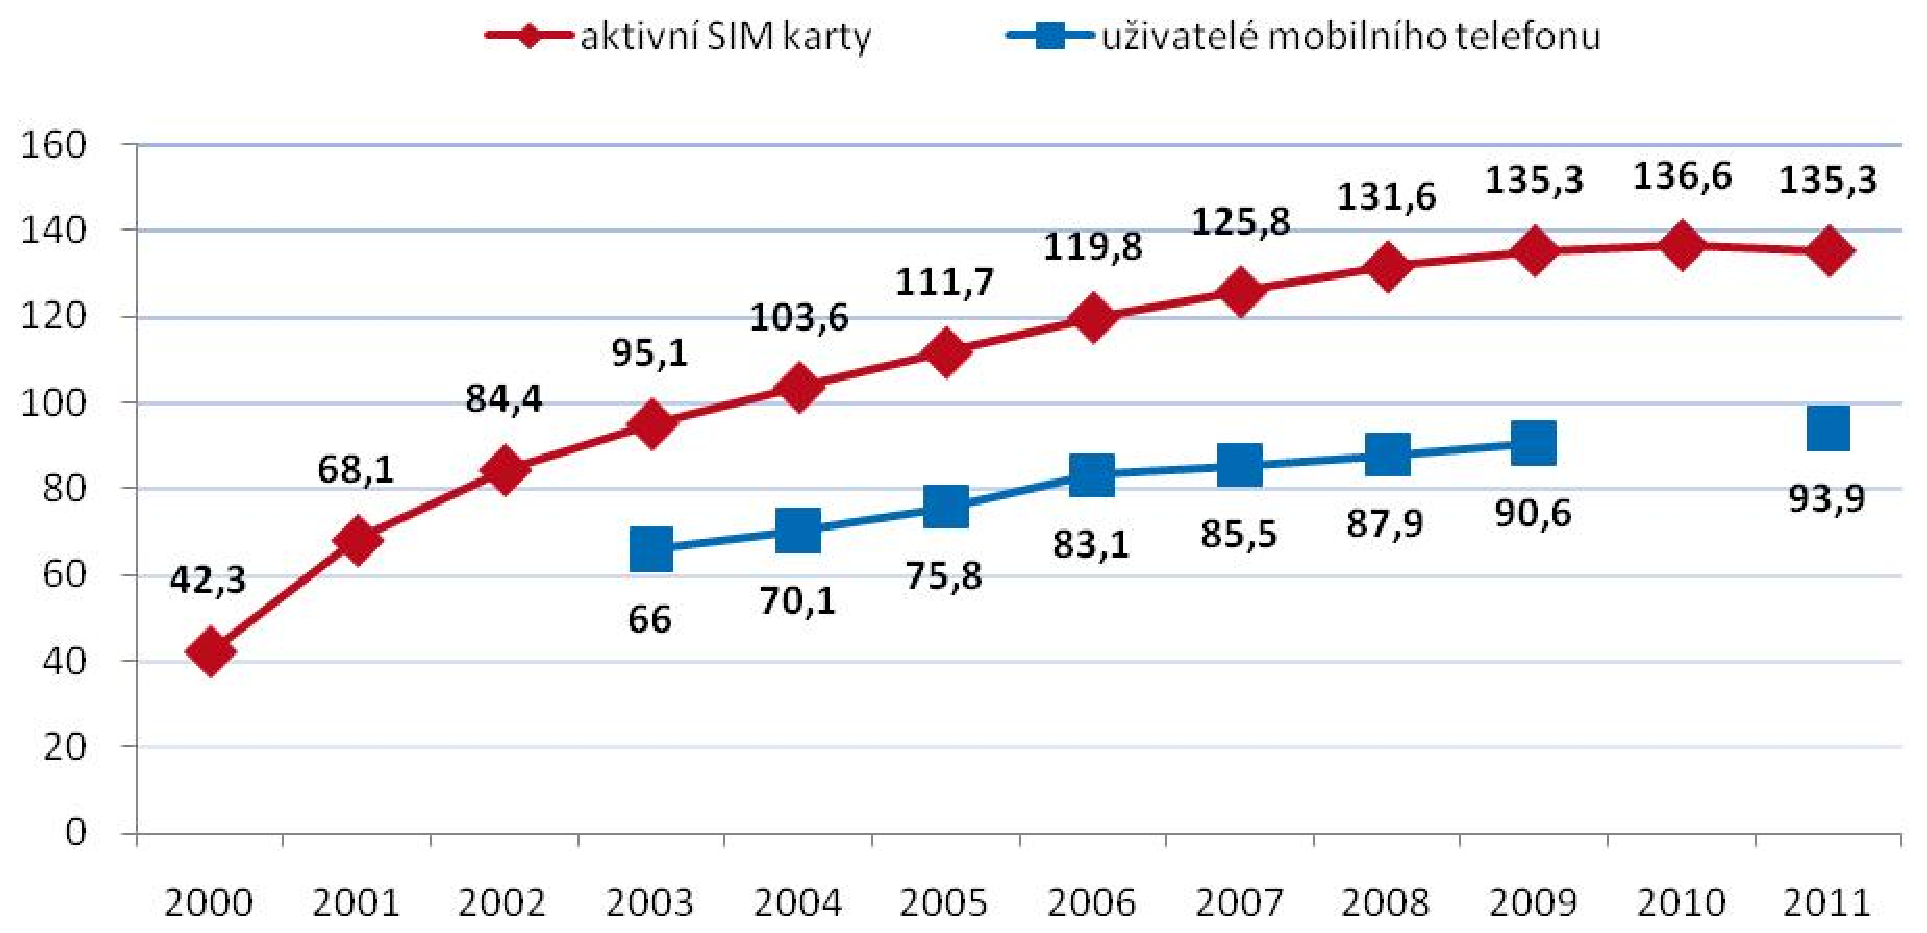
\includegraphics[scale=0.4]{graf_mobily_csu.eps}
\caption{Vývoj rozšíření mobilních telefonů v rámci populace ČR}
\label{fig:RozsireniMobil}
\end{figure}

\subsubsection{Smartphone}
Smartphone (česky „chytrý telefon“) v sobě kombinuje funkce mobilního telefonu a klasického počítače. Od klasických mobilních telefonů (tzv. „feature phone“) se smartphone liší v několika věcech:

\begin{enumerate}
	\item Přítomností pokročilého operačního systému (iOS, Android, Windows Phone/Mobile apod.)
	\item Přítomností lokálního úložiště, které může uživatel použít pro uložení vlastních dat.
	\item Možností připojit se telefonem k internetu a stahovat z něj data.
\end{enumerate}

Společnost Gartner definuje smartphone jako zařízení, které používá jasně rozpoznatelný operační systém umožňující vývojářům třetích stran vyvíjet pro tento systém aplikace (více o tom jak definujeme aplikace nastíní podkapitola \ref{Sec:Aplikace}). Aplikace třetích stran je možné instalovat a odstraňovat a při jejich vývoji je použito API daného operačního systému. Operační systém zajišťující fungování smartphone musí podporovat možnost používat více aplikací současně (tzv. multitasking) \cite{gartner_smartphone_definition}. 

Výrobci moderních smartphonů vybavili tento přístroj mnoha dalšími funkcemi. Mezi ty rozšířené patří například:

\begin{enumerate}
	\item fotoaparát/digitální kamera
	\item dotyková obrazovka s vysokým rozlišením
	\item možnost zaznamenávat zvuk
	\item GPS navigace
	\item přehrávač multimédií atd.
\end{enumerate}

\paragraph{Rozšíření smartphonů}
První zařízení, které můžeme označit pojmem smartphone (i když samotný termín ještě vymyšlen nebyl), bylo uvedeno na trh v roce 1994 pod označením „Simon Personal Communicator“, za jehož vývojem stála firma IBM \cite{simon}. Nabízel černobílý dotykový displej, který umožňoval ovládání přístroje prstem či stylusem a poskytoval uživatelům aplikace jako e-mailový klient, kalendář, hodiny a jednoduché hry. Vůbec poprvé termín „smartphone“ použila firma Ericsson při uvedení svého nového modelu GS88 s kódovým označením „Pandora“ \cite{history_of_the_smartphone}.

Mezi širokou veřejností je však za první smartphone považován až iPhone společnosti Apple, jehož první verze byla uvedena do prodeje v roce 2007 \cite{apple_unveils_iPhone}. Od momentu, kdy byl iPhone uveden na trh, zaznamenává podíl prodaných smartphonů ke klasickým telefonům (feature phone) dynamický růst. V roce 2011 tvořily, dle odhadů společnosti Ericsson, 30 \% prodaných mobilních telefonů smartphony, což činí oproti roku 2010 nárůst o 10 \% \cite{ericsson_report_web}. Celkový podíl používaných smartphonů ke klasickým telefonům je pak odhadován na 10 \%, tedy asi 1 miliarda zařízení \cite{ericsson_report_web}.

\paragraph{Významní výrobci}
Od uvedení prvních smartphonů na trh v druhé polovině devadesátých let vládla tomuto segmentu jednoznačně Nokia. Toto zaběhnuté paradigma se začalo pozvolna měnit až s příchodem iPhonu. Na grafu \ref{fig:VyrobciSmartphoneRozsireni}, který mapuje období mezi léty 2009–2012 je jasně vidět strmý pád Nokie a naopak vzestup konkurentů v podobě Applu, Samsungu a dalších.

\begin{figure}\centering
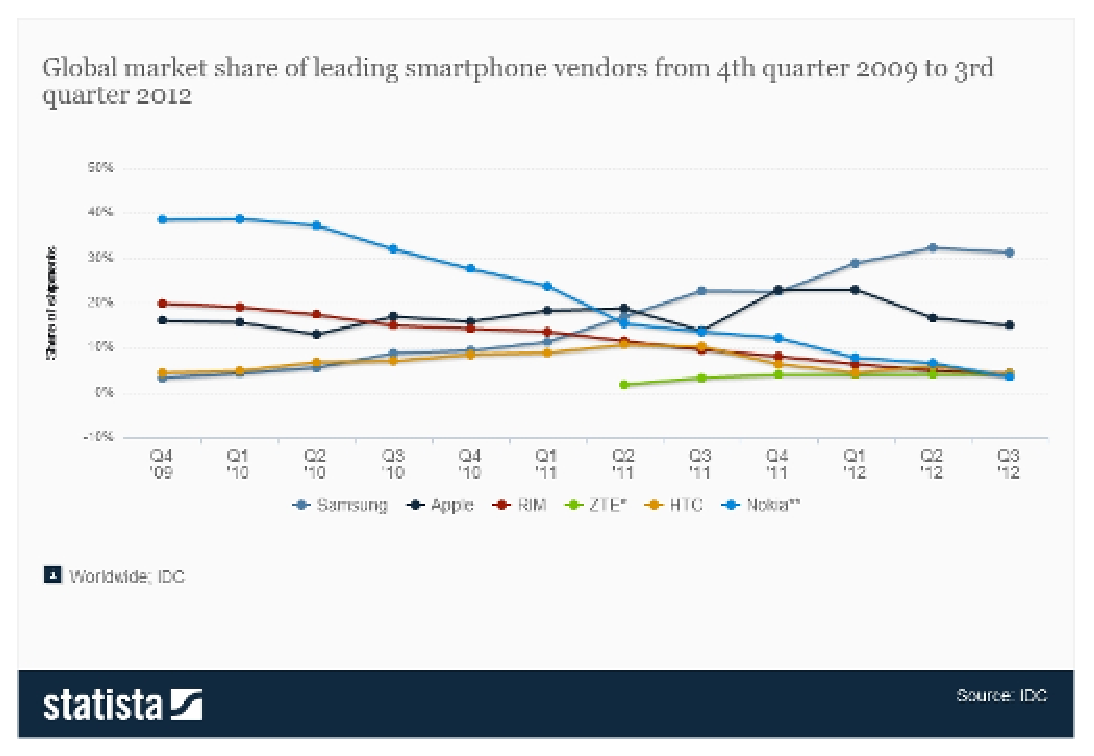
\includegraphics[width=1.0\textwidth]{smartphone_marketshare_vendors.eps}
\caption{Vývoj tržního podílu výrobců chytrých telefonů}
\label{fig:VyrobciSmartphoneRozsireni}
\end{figure}

Aktuální data z června roku 2012 ukazují zřetelnou převahu společnosti Samsung nad zbytkem trhu. Více než třetina dnes používaných smartphonů nese značku právě této společnosti. Oproti tomu zhruba polovičním podílem na trhu se může pochlubit společnost Apple. Původní hegemon – firma Nokia – nyní okupuje pouze lehce přes 6 \% tržního podílu.

\begin{figure}\centering
\includegraphics[width=0.6\textwidth]{smartphone_by_manufaturers.png}
\caption{Současný tržní podíl výrobců smartphonů na trhu}
\label{fig:VyrobciSmartphoneRozsireni2}
\end{figure}

\paragraph{Přehled mobilních platforem}
Řada zákazníků při výběru nového chytrého telefonu dbá nejen na vzhled a hardwarové parametry, ale důležitou roli při konečném rozhodování hraje i operační systém, který na přístroji běží. Někteří výrobci se snaží s konkrétním operačním systémem spojit svou značku (Apple, Nokia), jiní naopak dávají zákazníkům na výběr různé modely s různými systémy (HTC, Samsung).

\subparagraph{iOS}
iOS je produktem společnosti Apple, která jím vybavuje své produkty iPhone, iPod i iPad. Poprvé byl uveden v roce 2007 spolu se smartphonem iPhone na konferenci Macworld \cite{apple_unveils_iPhone}. Od té doby je neustále vylepšován a v současné době se již nachází ve verzi 6. Od dob první verze se však uživatelské prostředí iPhonu mění jen pozvolna. Apple, narozdíl od konkurence v podobě Androidu a Windows Phone, neumožňuje použití systému iOS na zařízeních, které nevyrobila firma Apple.

Celý koncept systému iOS je úzce spjat s velkým displejem smartphonu iPhone. Ovládání celého prostředí je uživateli umožněno pomocí celé řady multi-dotykových gest. Mezi nejznámější prvky z prostředí systému iOS můžeme zařadit tzv. „Home screen“, který pomocí matice ikon usnadňuje uživateli spouštění nainstalovaných aplikací. Dále stojí za zmínku například notifikační centrum, hlasové ovládání Siri nebo Game center.

\subparagraph{Android}
Operační systém Android byl původně vytvořen společností Android Inc., kterou v roce 2005 odkoupil gigant v oblasti internetového vyhledávání – firma Google \cite{google_buys_android}. Představení Androidu veřejnosti bylo úzce spjato se založením organizace Open Handset Alliance, která sdružovala výrobce software, hardware i telefonní operátory s cílem vyvinout otevřenou platformu a definovat nové standardy na poli mobilních telefonů \cite{android_announce}. Systém Android je šířen pod licencí Apache License a lze jej tedy označit za open-source software \cite{android_overview}.

Systém Android můžeme krom mobilních telefonů nalézt i na tabletech, chytrých televizích, herních konzolích a dalších zařízeních. Vysoká obliba Androidu mezi zákazníky pramení především z obrovského množství různých modelů, se kterými je tento systém na trhu nabízen. Vzhledem k otevřené licenci, pod kterou je systém šířen, je využíván širokým portfoliem výrobců, kteří tak ušetří za vývoj a správu vlastního systému.

Uživatelské rozhraní Androidu vzdáleně připomíná svého konkurenta iOS. Také zde najdeme „Home screen“, který je tvořen maticí ikon symbolizujících nainstalované aplikace. Stejně tak v Androidu můžeme nalézt třeba notifikační centrum. Od svých konkurentů se tato platforma odlišuje nepřeberným množstvím možností, jak upravit vzhled a chování systému.

\subparagraph{Windows Phone}
Windows Phone vznikl ve společnosti Microsoft jako odpověď na úspěch iOS a Androidu. Předešlý systém z dílmy redmondské firmy, Windows Mobile, již nebyl lákavý pro výrobce zařízení s velkými dotykovými obrazovkami. Microsoft tak představil počátkem roku 2010 na Mobile World Congress v Barceloně zcela nový operační systém, který nesl označení Windows Phone 7 \cite{ms_announce_wp}. Jeho uživatelské rozhraní tvořené velkými barevnými interaktivními dlaždicemi se na první pohled velmi liší od iOS a Androidu, avšak většinu principů práce s dotykovými zařízeními zachovává. 

Společnost Microsoft narozdíl od Applu či Google doposud nevyrábí vlastní chytré telefony a tak přijetí nové platformy bylo čistě na vůli výrobců telefonů. Na tomto poli se nový systém střetával především s Androidem, který je výrobcům k dispozici zdarma, zatímco Microsoft požaduje za použití Windows Phone licenční poplatky. Jako svůj hlavní systém si Windows Phone zvolila společnost Nokia, která se spolu s ním snaží dobýt zpět své ztracené pozice na trhu s chytrými telefony.

Od roku 2010, kdy byl systém poprvé představen, byl již několikrát vylepšen mnoha aktualizacemi, které přinášely do systému nové funkce (např. multitasking). Dva roky po uvedení systému Windows Phone Microsoft oznámil vydání nové verze svého systému pod názvem Windows Phone 8, která přináší přepracované jádro a některé nové funkce \cite{ms_unveils_wp8}.

\subparagraph{Firefox OS}
Firefox OS je mobilní operační systém, který je v současné době stále ještě ve vývoji a neběží tedy zatím na žádném reálně používaném zařízení. V této práci jej zmiňuji proto, že cíle, které si společnost Mozilla, jež stojí za tímto systémem, vytyčila, přímo korespondují s tématem této práce (více technických podrobností o Firefox OS naleznete v kapitole 2).

Vývoj systému Firefox OS byl oznámen v červnu 2011 v rámci komunity společnosti Mozilla. Celý projekt nesl kódové označení „Boot to Gecko“ a jeho cílem má být položení rovnítka mezi webové technologie a moderní mobilní telefony. V originální oznamovací zprávě se přímo říká \cite{booting_to_the_web}: „Chceme identifikovat překážky, které stěžují webovým vývojářům tvorbu aplikací, které budou v každém směru plnohodnotnými náhradami nativních aplikací pro platformy iOS, Android a WP7.“ První telefony s Firefox OS by se měly objevovat v prvním čtvrtletí roku 2013 \cite{ztes_first_firefoxos}.

\paragraph{Situace na trhu}
Podíváme-li se na aktuální situaci na trhu, můžeme jasně vidět, že na tomto poli nyní zcela zřetelně dominuje systém Android. Naopak dřívější hegemon Symbian, který poháněl zařízení společnosti Nokia, má již méně než 5 \% tržního podílu. iOS od Applu je pak druhým největším hráčem.

\begin{figure}\centering
\includegraphics[width=0.6\textwidth]{smartphone_by_platform.png}
\caption{Současný tržní podíl mobilních platforem}
\label{fig:MobilniPlatformyPodil}
\end{figure}

Další graf\ref{fig:MobilniPlatformyVyvoj} jasně ilustruje již zmíněné trendy. Můžeme zde vidět strmý propad Symbianu a naopak drtivý vzestup platformy Android, který od roku 2009 zaznamenala. 

\begin{figure}\centering
\includegraphics[width=1.0\textwidth]{graf_vyvoj_mobilnich_os.png}
\caption{Vývoj tržního podílu mobilních platforem}
\label{fig:MobilniPlatformyVyvoj}
\end{figure}

\section{Aplikace} \label{Sec:Aplikace}
\subsection{Obecná definice}
Definice aplikace (či aplikačního software) vychází z rozdílu mezi aplikací a programem či systémovým softwarem. Zatímco systémový software umožňuje chod hardwarového vybavení počítače a poskytuje ostatním programům prostředí k provádění úkonů, aplikace je program sloužící uživateli za nějakým jím požadovaným účelem. Dobrým příkladem takové aplikace je kupříkladu textový procesor či internetový prohlížeč.

V poslední době je slovo „aplikace“ spíše chápáno v jeho užším významu – jako aplikace pro mobilní zařízení. V angličtině bylo pro tyto účely odvozeno slovo „app“, které je zkráceninou slova „application“. Tímto zkrácením je mimo jiné reprezentován i co do funkčnosti užší záběr, kterým se mobilní aplikace vyznačují. Tento termín dokonce nabyl takové popularity, že byl v roce 2010 vyhlášen American Dialect Society „slovem roku“ \cite{app_word_of_the_year}.

\subsection{Mobilní aplikace}
Mobilní aplikaci definujeme jako samostatný software určený pro využití na smartphonech, tabletech a dalších přenosných zařízeních. Zpravidla jsou velmi úzce zaměřené na vykonání konkrétní činnosti a mají velmi málo funkcí (např. kalkulačka, internetový prohlížeč, čtečka RSS apod.).

Mobilní aplikace jsou převážně distribuovány přes takzvaná „tržiště“, kde uživatel najde kategorizovaný přehled aplikací, které si může pro svou platformu stáhnout (více o tržištích v podkapitole XY). Některé platformy podporují i možnost stahování mobilních aplikací prakticky odkudkoliv, například z webových stránek vývojáře, který aplikaci vytvořil (Android).

\subsubsection{Rozdělení mobilních aplikací}
Pro rozdělení mobilních aplikací můžeme využít v zásadě dva přístupy. Jedním z nich je rozdělit aplikace podle účelu, za nímž byly stvořeny. Další možností je potom rozdělit takové aplikace dle technologie, pomocí které byly vytvořeny.

\paragraph{Rozdělení dle účelu}
Při rozdělování aplikací dle účelu se musíme zaměřit na oblast činnosti, kterou má daná aplikace svému uživateli zpříjemnit. Níže jsem provedl jejich rozdělení dle účelu, při jehož tvorbě jsem vycházel z kategorizace, kterou pro rozdělení aplikací používají oficiální tržiště pro platformy iOS a Android.

\begin{enumerate}
	\item Hry
	\item Sociální sítě
	\item Multimédia – například aplikace na úpravu fotografií, přehrávání videa nebo hudby.
	\item Produktivita – GTD aplikace, time tracking apod.
	\item Komunikace – IM komunikátory, SMS aplikace apod.
	\item Doprava – GPS navigace, mapy apod.
	\item Cestování
	\item Kancelářské – zjednodušené verze kancelářských balíků, správa financí apod.
	\item Zábava
	\item. Nakupování – tipy, slevy apod.
	\item Informační – čtení zpráv, vzdělávání, počasí.
	\item Úpravy systému – rozšířené možnosti nastavení a úprav vzhledu.
	\item Životní styl – zdraví, jídlo.
	\item Sport – živé výsledky, informace.
\end{enumerate}

\paragraph{Dle technologie}
\subparagraph{Nativní aplikace}
Již ze slova „nativní“ v názvu této sekce plyne, že půjde o technologii, která je nějakým způsobem přirozená. V našem případě je to přirozenost technologie a chování aplikace k dané platformě. Pro vývoj mobilní aplikace pro konkrétní operační systém tedy používáme určitý programovací jazyk a určité nástroje. 

Nativní aplikace se většinou vyznačují dobrým výkonem a širokým spektrem funkcí. Vývojáři nativních aplikací mají totiž přístup k drtivé většině hardwarových i softwarových funkcí telefonu. I vzhled nativních aplikací je přesně takový, jaký ho uživatel očekává. Některé platformy mají totiž velmi striktní požadavky na vzhled jednotlivých ovládacích prvků (tlačítek, přechodů apod.) a nevyhovující aplikace vůbec nepřipouští na svá tržiště.

Nativní aplikace jsou většinou distribuovány přes oficiální tržiště konkrétní platformy. U operačního systému Android však můžeme pozorovat i jiné cesty, kterými uživatelé aplikace získávají (z webových stránek, neoficiální tržiště apod.). Více o vývoji nativních aplikací pro jednotlivé platformy si řekneme v kapitole 2.

\subparagraph{Webová aplikace}
Aplikaci označujeme jako webovou, pokud bylo při jejím vývoji použito tzv. webových technologií (např. HTML či JavaScript). Webová aplikace ke svému běhu potřebuje internetový prohlížeč nebo jeho jádro. Všeobecná rozšířenost webových aplikací pramení právě z tohoto faktu. Internetový prohlížeč je totiž předinstalován na všech známých operačních systémech (desktopových i mobilních) a díky tomu je velmi široce rozšířený.

V prostředí mobilních telefonů nacházejí webové aplikace uplatnění zejména díky nízkým nákladům na vytvoření a jejich multiplatformnosti. Webová aplikace na mobilním telefonu může mít buď formu webové stránky uzpůsobené pro zobrazení na malých displejích či offline aplikace, která ke svému běhu nevyžaduje internetové připojení.

Velkým nedostatkem, jímž webové aplikace trpí, je jich omezená funkcionalita. Webové aplikace nemohou přistupovat k žádným specifickým funkcím telefonu vyjma samotného internetového prohlížeče. Proto se webové aplikace využívají především jako zobrazovač obsahu, který je formátován pro snadnou konzumaci na mobilním telefonu.

\subparagraph{Hybridní aplikace}
Definice hybridních aplikací není zatím úplně přesně vymezená. Pokud bych se měl pokusit takovou aplikaci definovat, tak se jedná o aplikaci, pro jejíž vývoj bylo použito převážně webových technologií, avšak hybridní aplikace umožňuje uživateli využívat některé hardwarové i softwarové funkce telefonu stejně, jako by se jednalo o aplikaci nativní.

Hybridní aplikace se navenek tváří stejně jako aplikace nativní, takže většinou splňují všechny požadavky, které si kladou oficiální tržiště. Uživatel si pak takovou aplikaci stáhne aniž by věděl, že nebyla vyvinuta v nativním kódu. Více o hybridních aplikacích se dozvíte v kapitolách 3, 4 a 5. % TODO reference

\subsubsection{Popularita mobilních aplikací}
Chytré telefony byly ve svých počátcích populární zejména díky přístupu na internet přes webový prohlížeč. Dnes však tomuto světu začínají pozvolna vládnout aplikace. Průměrný uživatel smartphonu měl v roce 2012 na svém zařízení nainstalováno 41 aplikací, přičemž o rok dříve to bylo jen 32 \cite{mobile_app_usage_statistics}. Tento strmý vzestup dobře ilustruje i poměr, v jakém uživatelé využívají internetový prohlížeč oproti staženým aplikacím. V roce 2012 bylo poprvé zaznamenáno, že uživatelé používali pro přístup k obsahu více stažené aplikace než internetový prohlížeč. V květnu 2012 byl tento poměr 51,1 \% ku 49,8 \% ve prospěch aplikací \cite{comscore_report_may}.

Popularita mobilních aplikací je založena na několika faktorech. Jedním z nich je nepopiratelně jejich nízká cena. Mobilní aplikace v Apple App Store stojí v lednu 2013 průměrně 1,61 \$ \cite{app_store_metrics}. Za takto nízkou cenu se většině uživatelů vyplatí, především z důvodu pohodlí, aplikaci zakoupit, než podstupovat poměrně složitý proces odemčení telefonu a následného nahrávání aplikací nelegálně stažených z internetu. Tento fakt je v ostrém kontrastu s prostředím desktopových aplikací, které často stojí tisíce korun a pro mnoho lidí jsou z tohoto důvodu nedostupné a ti se poté uchylují k pořizování pirátských kopií tohoto software.

Dalším faktorem, který zapříčiňuje popularitu aplikací, je nepochybně pohodlí při jejich obstarávání. Uživatelé platformy Windows byli po léta zvyklí, že software pro svůj počítač museli stahovat z různých (často pochybných) zdrojů. Vyžadovalo to od nich zvýšené úsilí s často neuspokojivým výsledkem. Oficiální distributoři mobilních aplikací se snaží toto úsilí redukovat na minimum. Každá platforma má své oficiální tržiště, kde dělí uživatele od získání jeho aplikace doslova jediný klik. Díky tomu mohou vývojáři oslovovat obrovskou masu uživatelů a držet tak cenu svých aplikací velmi nízko.

Třetím a možná nejdůležitějším faktorem je přirozeně velice příznivé prostředí pro vývojáře. Společnosti stojící za vývojem jednotlivých platforem si svou komunitu developerů značně hýčkají. Krom pečlivé dokumentace mají připravené i specializované nástroje, kterými vývoj nativních aplikací pro své platformy usnadňují. Navíc díky výše zmíněné jednoduchosti finální distribuce se vývojář nemusí příliš zabývat s marketingem kolem své aplikace. O příznivém prostředí pro vývojáře svědčí i fakt, že od spuštění Apple App Store jim bylo za prodej placených aplikací vyplaceno více než 5 miliard dolarů \cite{comscore_report_may}.

Zajímavý je také pohled na nejpopulárnější aplikace na jednotlivých platformách. Obecně jsou mezi uživateli oblíbené mapy, klienti pro sociální sítě či e-mail nebo novinky o počasí.

\paragraph{Nejpopulárnější aplikace pro platformu Android \cite{desitka_nej_aplikaci_android}}
\begin{enumerate}
	\item Google Search
	\item Gmail
	\item Facebook
	\item Google Maps
	\item YouTube
	\item Pandora
	\item Twitter
	\item Adobe Reader
	\item Advanced Task Killer
	\item The Weather Channel
\end{enumerate}

\paragraph{Nejpopulárnější aplikace pro platformu iOS \cite{desitka_nej_aplikaci_android}}
\begin{enumerate}
	\item Maps
	\item Facebook
	\item YouTube
	\item Stocks
	\item Weather
	\item Facebook Messenger
	\item The Weather Channel
	\item Twitter
	\item Pandora
	\item Instagram
\end{enumerate}

Samostatným segmentem trhu jsou firmy a jejich vztah k mobilním aplikacím. Velké i malé firmy používají aplikaci ke komunikaci se svými zákazníky a to z několika hledisek. Jednak je to pro ně skvělý marketingový kanál. Přes specializované aplikace ke svým produktům či službám mohou oslovovit cílovou skupinu, která má o jejich produkty zájem a nabídnout jim něco navíc. Nenahánějí tedy zajíce v pytli, ale cílí na uživatele, kteří projevili o jejich aplikaci (a potažmo produkt) zájem. Mohou jim pak šít nabídky přímo na míru, poskytovat speciální slevy a podobně. Zajímavým benefitem pro uživatele je i poskytnutí podrobných informací o produktech, usnadnění jejich nákupu či komunikace s firmou. Podle některých předpovědí bude mobilní aplikace pro firmy do budoucna stejně důležitý komunikační kanál, jakou je dnes třeba e-mailová adresa či telefon \cite{forbes_business_checklist}.

\subsubsection{Distribuční platformy}
\paragraph{Apple App Store}
Oficiální tržiště s aplikacemi pro systém iOS bylo spuštěno v roce 2008 společně s modelem iPhone 3GS. V lednu 2013 se na něm nacházelo 774 425 aplikací dostupných ke stažení \cite{app_store_metrics}. Od spuštění App Store se již počet stažených aplikací vyšplhal na 30 miliard \cite{mobile_app_usage_statistics} a vývojářům, kteří své aplikace poskytují za peníze, bylo dohromady vyplaceno 5 miliard dolarů \cite{mobile_app_usage_statistics}.

Vývojáři, kteří chtějí na App Store publikovat své aplikace, musí dodržet řadu podmínek na funkčnost a vzhled svých aplikací, které si Apple klade. Cílem těchto restrikcí je předejít distribuci aplikací pochybné kvality, které by kazily pověst celé platformě. V důsledku těchto restrikcí je přístup do App Store odepřen nejen aplikacím jejichž vzhled neodpovídá zvyklostem platformy iOS, ale i aplikacím, které svou funkčností nepřináší nic navíc oproti webovým stránkám. V App Store tedy není možné publikovat obyčejné webové aplikace.

Pokud chce vývojář své aplikace prodávat v App Store, musí se smířit s tím, že 30 \% z každé prodané aplikace jde na účet Applu \cite{distribute_your_app_ios}, 70 \% pak zůstává vývojáři. Průměrná cena (neherní) aplikace v App Store je 1,61 \$, průměrná hra vás pak přijde na 0,91 \$ \cite{app_store_metrics}. Nejpopulárnější kategorií v App Store jsou jednoznačně hry, kde naleznete více jak 130 000 aplikací. V závěsu jsou pak kategorie Vzdělání, Zábava, Životní styl a Knihy \cite{app_store_metrics}. Nejpopulárnější placenou aplikací je hra Angry Birds, z aplikací nabízených zdarma je to oficiální klient pro sociální síť Facebook \cite{apple_names_top_apps}.

\paragraph{Google Play}
Obdoba App Store pro platformu Android je tržiště Google Play, dříve známé pod názvem Android Market. Ten byl spuštěn v roce 2008 a o rok později do něj byla přidána podpora pro prodej placených aplikací. V současné době se na Google Play nachází přibližně 700 000 aplikací \cite{google_says_700k_apps}.

Podmínky pro vývojáře placených aplikací jsou podobné jako u Applu. Přímo vývojáři plyne 70 \% z každé prodané aplikace, zbytek putuje na účty partnerů Googlu \cite{transaction_fees_android}. Při publikování aplikací na Google Play platí pro vývojáře mnohem mírnější pravidla než v App Store. Tento fakt je terčem některých kontroverzí, neboť se díky tomu na Google Play dostávají i aplikace nevalné kvality a dokonce zavirované aplikace, které mohou poškodit telefon uživatele \cite{new_android_trojan}. Na druhou stranu tento přístup poskytuje vývojářům i uživatelům větší svobodu při tvorbě i výběru aplikací.

\paragraph{Windows Phone Store}
Stejně jako Google či Apple, i Microsoft má oficiální tržiště pro svou plaftormu Windows Phone. Windows Phone Store byl spuštěn spolu s uvedením první řady operačního systému Windows Phone v říjnu 2010. Ze tří předních platforem je ve Windows Phone Store dostupný jasně nejnižší počet aplikací – v roce 2012 jich bylo 100 000 \cite{mobile_app_usage_statistics}. Zhruba 7x nižší číslo oproti konkurenčním tržištím je zapříčiněno především dvouletým zpožděním, které platforma Windows Phone má oproti konkurenci.

Microsoft se při tvorbě svého tržiště inspiroval u Applu a zavedl podobně přísná pravidla pro schvalování aplikací, které chce vývojář na tržišti nabízet. I zde je velmi dbáno na vzhled, chování a obsah aplikací. Podobně jako konkurence přistupuje i Microsoft k rozdělení podílu z každé prodané aplikace – 30 \% jde Microsoftu, 70 \% vývojáři \cite{wp_right_mix}.

% TODO dodělat chybějící literaturu